\chapter{Selectividad interruptores automáticos de baja tensión}
En caso de defecto debe abrir el interruptor automático situado inmediatamente aguas arriba del defecto y sólo él.
\begin{figure}[H]
	\centering
	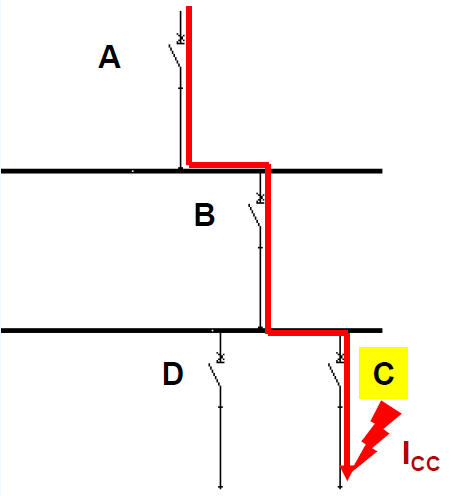
\includegraphics[width=0.4\linewidth]{Images/18}
\end{figure}
\section{Selectividad Total}
Para cualquier valor de la intensidad de defecto “aguas abajo” de B, el interruptor automático B es el único en desconectar 
\section{Selectividad Parcial}
Para ciertos valores de la intensidad de defecto “aguas abajo” de B, el interruptor B es el único en desconectar, pero para otros abren los dos interruptores, A y B
\section{Selectividad frente a sobrecargas}
Se deben cumplir dos condiciones:
\begin{enumerate}
	\item Corriente de sobrecarga
	\begin{equation}
		I_{tDQ2}< I_{tNDQ1} \rightarrow 1.45 I_{NQ2} < 1.13 I_{NQ1}
	\end{equation}
	\item Diferencia de tiempos mínima de 1 s
	\begin{equation}
		t_{tDQ2}+1s\le t_{tNDQ1}
	\end{equation}
\end{enumerate}
\begin{figure}[H]
	\centering
	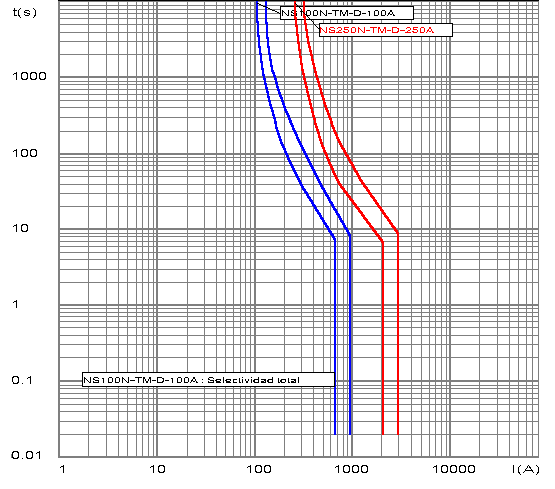
\includegraphics[width=0.5\linewidth]{Images/19}
\end{figure}

\section{Selectividad frente a cortocircuitos}
Se deben cumplir 2 condiciones:
\begin{enumerate}
	\item Condición de selectividad amperimétrica
	\begin{equation}
		I_{iDQ2}< I_{iNDQ1} 
	\end{equation}
	\item Condición de intensidad límite de selectividad $I_s=I_{iNDQ1}$
	\begin{equation}
		I_{kB_{min}Q2}< I_s
	\end{equation}
\end{enumerate}

Se dice que existe selectividad total si la intensidad de no disparo de Q1 es mayor que el cortocircuito máximo en Q2:
\begin{equation}
	I_{kB_{max}Q2}< I_s
\end{equation}
\section{Selectividad frente a cortocircuitos moderados}
Se deben cumplir 4 condiciones:
\begin{enumerate}
	\item Dispersión características retardo corto:
	\begin{equation}
		I_{mDQ2}\le I_{mNDQ1}
	\end{equation}
	\item Tiempo escalonamiento: 
	\begin{itemize}
		\item Para relés electrónicos: 
		\begin{equation}
			t_e \ge 70 ms
		\end{equation}
		\item Para relés electromecánicos:
		\begin{equation}
			t_e \ge 100 ms
		\end{equation}
	\end{itemize}
	
	\item Cortocircuito máximo:
	\begin{equation}
		I_{kB_{max}Q2}< I_{cwQ1}
	\end{equation}
	\item Disparo instantáneo:
	\begin{equation}
		I_{kB_{min}Q2}< I_{iNDQ1} 
	\end{equation}
\end{enumerate}
\begin{figure}[H]
	\centering
	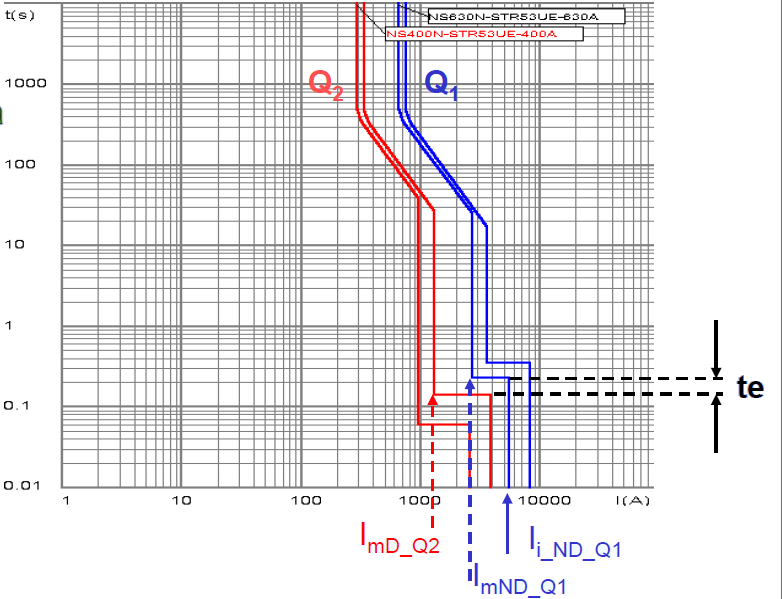
\includegraphics[width=0.5\linewidth]{Images/20}
\end{figure}

\section{Coordinación entre interruptores automáticos}
Instalación en serie de dos interruptores automáticos coordinados de forma que el preconectado ayude al postconectado al despeje de cortos fuertes para reducir el poder de corte del interruptor a la salida. 
\begin{itemize}
	\item Para cortocircuitos moderados el interruptor aguas abajo abre y el aguas arriba no abre
	\item Para cortocircuitos elevados el interruptor aguas arriba ayuda a la apertura de la falta
\end{itemize}

Para que pueda darse esta situación se debe cumplir que el interruptor de cabecera y el embarrado deben soportar térmicamente los cortocircuitos.
\newline

Se usa en instalaciones con continuidad de servicio no imperativa.
\newline

 Tiene las siguientes ventajas:
 \begin{itemize}
 	\item Bajo nivel de costes
 
 	\item Dimensiones mínimas del equipo eléctrico
 	
 	\item En caso de ampliaciones, puede permitir mantener parte de las instalaciones existentes
 \end{itemize}
\section{Selectividad lógica}
Se emplea un circuito con un sistema de control con microcontrolador que realiza las siguientes operaciones:
\begin{itemize}
	\item Identifica el interruptor al que corresponde la eliminación de la falta
	\item Reduce el tiempo de disparo del interruptor seleccionado
	\item Conserva la coordinación selectiva de los interruptores situados aguas arriba
	\item 	El límite de selectividad final que puede obtenerse es $I_{cw}$
	\item	Requiere relés electrónicos en todos los interruptores 
\end{itemize}